
Let \begin{equation}
  f(x,y)=3(x-5)^4+10(y-9)^2
  \label{eq:f}
\end{equation}
and 
\begin{equation}
  g(x,y)=\max(x-5,0)+10|y-9|
  \label{eq:g}
\end{equation}


Clearly, the minimum of both $f(x,y)$ and $g(x,y)$ is $0$ and they both minimized by $x=5$, $y=9$.

The Polyak step size is \begin{equation}
  \alpha_{\text{Polyak}}=\frac{f(x)-f^*}{\del f(x)^T\del f(x)}
  \label{eq:polyak-step}
\end{equation}
where $x$ is the parameter vector, $f(x)$ is the function to optimise, and $f^*\approx\min_xf(x)$.

\begin{figure}
  \begin{center}
    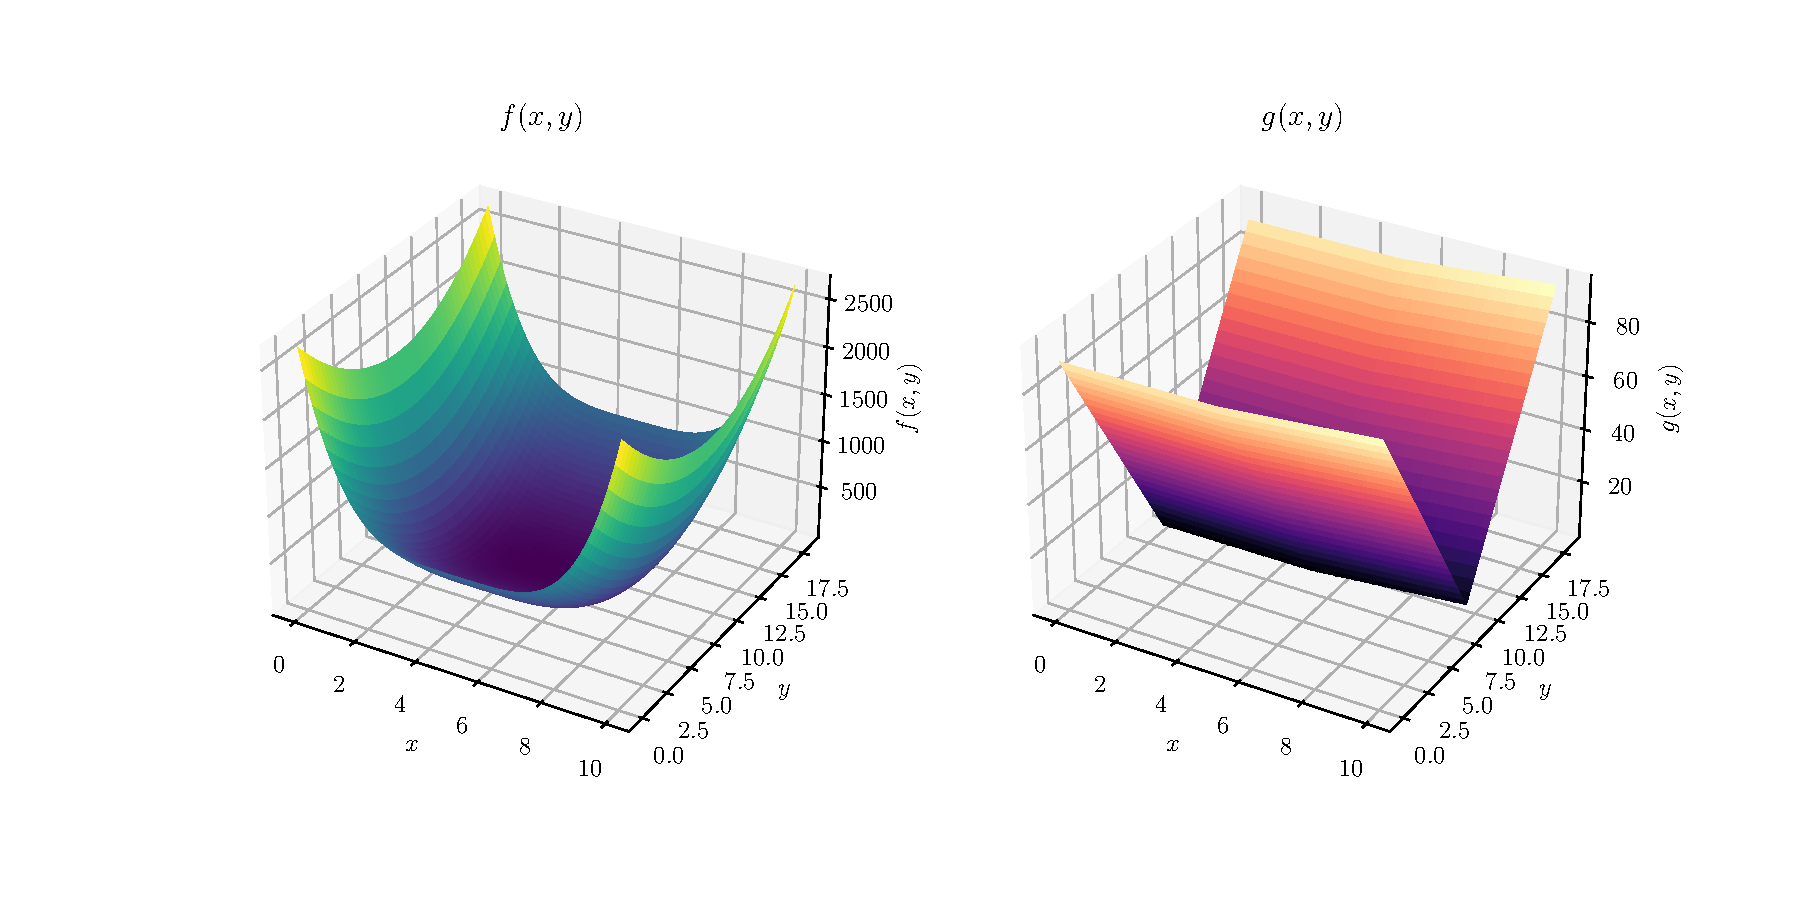
\includegraphics[width=0.95\textwidth]{fig/f-g.pdf}
  \end{center}
  \caption{}\label{fig:f-and-g}
\end{figure}

